\begin{comment}

\begin{figure*}[t!]
    \centering
    \scriptsize
\begin{tabular}{cl|@{}l}
\multicolumn{3}{c}{\textbf{Constraints:} \boldsymbol{$\ \ \ C_n: 0\leq i < N, \ \ \ \ \ \ C_m: 0\leq j < M, \ \ \ \ C_{m'}: 1\leq j < M, \ \ \ \ C_{k}: 0\leq k < 2$}}
\\\hline
  &
    \ \ \ \ \ \ \ \ \ \ \ \ \ \ \ \ \ \ \ \ \ \ \ 
    \textbf{Generated Code (different versions)}
  &
    \ \ \ \ \ \ \ \ \ \ \ \ \ \  
    \textbf{\framework representation (Layer I, Layer II and Layer III)}
\\\hline

{\textbf{\normalsize(a)}} &
\begin{lstlisting}[language=C,escapechar=@]
float b1[M], b2[M], out[N][M], avg[N][M]
a = 1.5
for (i in 0..N)
  for (j in 0..M)
    b1[j] = a*f1[i,j]@\label{fig:motivating:code1:stmt1}@
  for (j in 0..M)
    b2[j] = a*f2[i,j]@\label{fig:motivating:code1:stmt2}@
  for (j in 0..M)
    out[i,j] = b1[j] & b2[j]@\label{fig:motivating:code1:stmt3}@
for (i in 0..N)
  for (j in 1..M)
    avg[i,j] = (out[i,j-1] + out[i,j])/2
\end{lstlisting} 
    &  
\begin{tabular}{c|l}
\multirow{5}{*}{\textbf{Layer I}}
    & {\boldsymbol{$\{a(0)\} $}}: $\ 1.5$\\
    & {\boldsymbol{$\{b_1\ (i, j): C_n \wedge C_m\} $}}: $\ a(0)*f_1(i,  j)$  /* $C_n$ and $C_m$ are defined above. */ \\       
    & {\boldsymbol{$\{b_2\ (i, j): C_n \wedge C_m\}$}}: $\ a(0)*f_2(i,  j)$ \\
    & {\boldsymbol{$\{out(i, j): C_n \wedge C_m\}$}}: $\ b_1(i, j) \ \&\ b_2(i, j)$ \\
    & {\boldsymbol{$\{avg(i, j): C_n \wedge C_{m'}\}$}}: $(out(i,j-1) + out(i,j))/2$\\\hline
\multirow{5}{*}{\textbf{Layer II}}
    & $\{\ \ a[0]\} : \ 1.5$  \\
    & $\{\ b_1[1, i, 0, j]: C_n \wedge C_m\}: a[0]*f_1[i, j]$ /* $C_n$ and $C_m$ are defined above. */ \\
    & $\{\ b_2[1, i, 1, j]: C_n \wedge C_m\}: a[0]*f_2[i, j]$ \\
    & $\{out[1, i, 2, j]: C_n \wedge C_m\}: b_1[1,i,0,j] \ \&\ b_2[1,i,1,j]$ \\
    & $\{avg[2, i, j]: C_n \wedge C_{m'}\}: (out[1,i,2,j-1] + out[1,i,2,j])/2$ \\\hline
\multirow{8}{*}{\textbf{Layer III}}
    & Layer II representation + the following data \ mapping\\
    & $\{\ \ a[0] \rightarrow scalar_{0}\}$\\
    & $\{\ b_1[1, i, 0, j] \rightarrow buf_{b1}[j]:  C_n \wedge C_m \}$ /* $C_n$ and $C_m$ are defined above. */ \\
    & $\{\ b_2[1, i, 1, j] \rightarrow buf_{b2}[j]:  C_n \wedge C_m\}$\\
    & $\{out[1, i, 2, j] \rightarrow buf_{out}[i,j]:  C_n \wedge C_m\}$\\
    & $\{avg[2, i, j] \rightarrow buf_{avg}[i,j]:  C_n \wedge C_{m'} \}$\\
\end{tabular}
    \\\hline
{\textbf{\normalsize(b)}} &
\begin{lstlisting}[language=C,escapechar=@]
float b1[N][M], b2[N][M], out[N][M],
      avg[N][M]
a = 1.5
parallel for (i in 0..N)
  for (j in 0..M)
    b1[i, j] = a*f1[i,j]
  for (j in 0..M)
    b2[i, j] = a*f2[i,j]
  for (j in 0..M)
    out[i,j] = b1[j] & b2[j]
for (i in 0..N)
  for (j in 1..M)
    avg[i,j] = (out[i,j-1] + out[i,j])/2
\end{lstlisting}
    & 
\begin{tabular}{c|l}
 \multirow{3}{*}{\textbf{Layer I }}  & \\ & Same as (a) Layer I\\ \\\hline
 \multirow{6}{*}{\textbf{Layer II}}
     & $\{\ \ a[0]\} : \ 1.5$  \\
    & $\{\ b_1[1, i (cpu, virtual), 0, j]: C_n \wedge C_m\}: a[0]*f_1[i, j]$ \\
    & $\{\ b_2[1, i (cpu, virtual), 1, j]: C_n \wedge C_m\}: a[0]*f_2[i, j]$ \\
    & $\{out[1, i (cpu, virtual), 2, j]: C_n \wedge C_m\}: b_1[1,i,0,j] \ \&\ b_2[1,i,1,j]$ \\
    & $\{avg[2, i (cpu, virtual), j]: C_n \wedge C_{m'}\}: (out[1,i,2,j-1] + out[1,i,2,j])/2$ 
 \\\hline
 \multirow{6}{*}{\textbf{Layer III}}
    & Layer II representation + the following data \ mapping\\        
    & $\{\ \ a[0] \rightarrow scalar_{0}\}$\\
    & $\{\ b_1[1, i (cpu, virtual), 0, j] \rightarrow buf_{b1}[i,j]:  C_n \wedge C_m \}$\\
    & $\{\ b_2[1, i (cpu, virtual), 1, j] \rightarrow buf_{b2}[i,j]:  C_n \wedge C_m\}$\\
    & $\{out[1, i (cpu, virtual), 2, j] \rightarrow buf_{out}[i,j]:  C_n \wedge C_m\}$\\
    & $\{avg[2, i (cpu, virtual), j] \rightarrow buf_{avg}[i,j]:  C_n \wedge C_{m'} \}$\\
\end{tabular}  
    \\\hline
{\textbf{\normalsize(c)}} &
\begin{lstlisting}[language=C]
float b1[N][M], b2[N][M], out[N][M],
      avg[N][M]
a = 1.5
parallel for (i in 0..N)
  for (j in 0..M)
    b1[i,j] = a*f1[i,j]
    b2[i,j] = a*f2[i,j]
    out[i,j] = b1[i,j] & b2[i,j]
for (i in 0..N)
  for (j in 1..M)
    avg[i,j] = (out[i,j-1] + out[i,j])/2
\end{lstlisting}
    & 
\begin{tabular}{c|l}
 \multirow{3}{*}{\textbf{Layer I }}  & \\ & Same as (a) Layer I\\ \\\hline
 \multirow{5}{*}{\textbf{Layer II}}
    & $\{\ \ a[0]\} : \ 1.5$\\
    & $\{\ b_1[1, i (cpu, virtual), j, 0]: C_n \wedge C_m\}: a[0]*f_1[i, j]$\\
    & $\{\ b_2[1, i (cpu, virtual), j, 1]: C_n \wedge C_m\}: a[0]*f_2[i, j]$\\
    & $\{out[1, i (cpu, virtual), j, 2]: C_n \wedge C_m\}: b_1[1,i,j,0] \ \&\ b_2[1,i,j,1]$\\
    &$\{avg[2, i (cpu,virtual), j]:C_n\wedge C_{m'}\}:(out[1,i,j-1,2]+out[1,i,j,2])/2$\\\hline
 \multirow{8}{*}{\textbf{Layer III}}
    & Layer II representation + the following data \ mapping\\
    & $\{a\ [0] \rightarrow scalar_{0}\}$\\
    & $\{b_1\ [1, i (cpu, virtual), j, 0] \rightarrow buf_{b1}[i,j]:  C_n \wedge C_m \}$\\
    & $\{b_2\ [1, i (cpu, virtual), j, 1] \rightarrow buf_{b2}[i,j]:  C_n \wedge C_m\}$\\
    & $\{out[1, i (cpu, virtual), j, 2] \rightarrow buf_{out}[i,j]:  C_n \wedge C_m\}$\\
    & $\{avg[2, i (cpu, virtual), j] \rightarrow buf_{avg}[i,j]:  C_n \wedge C_{m'} \}$\\
 \end{tabular}
\\\hline
{\textbf{\normalsize(d)}} & 
\begin{lstlisting}[language=C,escapechar=@]
float out[N][M], avg[N][M]
a = 1.5
parallel for (i in 0..N)
  for (j in 0..M)
    float t1 = a*f1[i,j]
    float t2 = a*f2[i,j]
    out[i,j] = t1 & t2
for (i in 0..N)
  for (j in 1..M)
    avg[i,j] = (out[i,j-1] + out[i,j])/2
\end{lstlisting}
    &    

\begin{tabular}{c|l}
 \multirow{3}{*}{\textbf{Layer I }}  & \\ & Same as (a) Layer I\\ \\\hline
 \multirow{3}{*}{\textbf{Layer II}}  & \\ & Same as (c) Layer II\\ \\\hline
 \multirow{8}{*}{\textbf{Layer III}}
    & Layer II representation + the following data \ mapping\\
    & $\{\ \ \ a[0] \rightarrow scalar_{0}\}$\\
    & $\{\ \ b_1[1, i (cpu, virtual), j, 0] \rightarrow scalar_{1}:  C_n \wedge C_m \}$\\
    & $\{\ \ b_2[1, i (cpu, virtual), j, 1] \rightarrow scalar_{2}:  C_n \wedge C_m\}$\\
    & $\{out[1, i (cpu, virtual), j, 2] \rightarrow buf_{out}[i,j]:  C_n \wedge C_m\}$\\
    & $\{avg[2, i (cpu, virtual), j, 0] \rightarrow buf_{avg}[i,j]:  C_n \wedge C_{m'} \}$\\   
 \end{tabular} 
    \\\hline
{\textbf{\normalsize(e)}} &
\begin{lstlisting}[language=C,escapechar=@]
float b1[N][2], b2[N][2], out[N][2],
      avg[N][M];
a = 1.5
parallel for (i in 0..N)
  for (j in 0..M)
    for (k in 0..2)
      b1[i,k] = a*f1[i,j-1+k]@\label{fig:motivating:code4:stmt1}@
    for (k in 0..2)
      b2[i,k] = a*f2[i,j-1+k]
    for (k in 0..2)
      out[i,k] = b1[i,k] & b2[i,k]@\label{fig:motivating:code4:stmt3}@
    if (j > 0)  
      avg[i,j] = (out[i,0] + out[i,1])/2
\end{lstlisting}
    & 
\begin{tabular}{c|l}
 \multirow{3}{*}{\textbf{Layer I }}  & \\ & Same as (a) Layer I\\ \\\hline
 \multirow{8}{*}{\textbf{Layer II}}
    & $\{\ \ a[0]\}: 1.5$\\
    & $\{b_1\ [1, i (cpu, virtual),  j, 0, k]: C_n \wedge C_m \wedge C_k\}: a[0]*f_1[i, j-1+k]$\\
    & $\{b_2\ [1, i (cpu, virtual),  j, 1, k]: C_n \wedge C_m \wedge C_k\}: a[0]*f_2[i, j-1+k]$\\
    & $\{out[1, i (cpu, virtual), j, 2, k]: C_n \wedge C_m \wedge C_k\}: b_1[1,i,j,0,k] \ \&\ b_2[1,i,j,1,k]$\\
    & $\{avg[1, i (cpu, virtual), j, 3, 0]: C_n \wedge C_{m'}\ \ \ \ \ \ \ \ \ \}: (out[1,i,j,2,0] + out[1,i,j,2,1])/2$ \\
    \hline
 \multirow{8}{*}{\textbf{Layer III}}
    & Layer II representation + the following data \ mapping\\
    & $\{a\ [0] \rightarrow scalar_0\}$\\        %
    & $\{b_1\ [1, i (cpu, virtual), j, 0, k] \rightarrow buf_{b1}[i,k]:  C_n \wedge C_m \wedge C_k\}$ \\
    & $\{b_2\ [1, i (cpu, virtual), j, 1, k] \rightarrow buf_{b2}[i,k]:  C_n \wedge C_m \wedge C_k\}$ \\
    & $\{out[1, i (cpu, virtual), j, 2, k] \rightarrow buf_{out}[i,k]:  C_n \wedge C_m \wedge C_k\}$\\
    & $\{avg[1, i (cpu, virtual), j, 3, 0] \rightarrow buf_{avg}[i,j]:  C_n \wedge C_{m'} \}$\\        %
 \end{tabular} 
    \\
    \end{tabular}
    \caption{Resulting code and the three layers of representation for 
    (a) Unoptimized code implementing the motivating example,
    (b) Full expansion of b1 and b2 to allow parallelism,
    (c) Loop fusion,
    (d) Contraction of b1 and b2 to scalars, and 
    (e) Further fusion with redundant computation. }
    \label{fig:example-ir}
\end{figure*}
\end{comment}

%%%%%%%%%%%%%%%%%%%%%

%\begin{itemize}
%  \item A three-level IR that separates the algorithm from the schedule and the data-layout. Since the memory-layout is not represented in the high levels of the IR where scheduling happens, reasoning about code transformations is easier since it does not involve data-layout transformations as well.
  %, since code transformation passes do not need to transform the data layout.  The third level specifies the data-layout.
  %The first level describes the computations without describing how these computations are scheduled or where they are stored.  The second level describes how computations are scheduled but does not represent how they are stored.  
%  \item The framework allows the user to use an affine transformation or a non-affine transformation to transform the iteration domain to the time-space domain.
%  \item A code generator that takes as input the time-space representation regardless of whether it was generated using an affine or a non-affine transformation; it generates a sequence of loop nests as output.
%  \item An open source framework that implements the three-level IR and generates code targeting single core CPU, multi-core CPU with vectorization and targets GPU architectures.  This framework is validated on the Halide industrial DSL compiler.
%\end{itemize}

%%%%%%%%%%%%%%%%%%%%%%%%%%%%%%%%%%%%%%%%%%%%%%%%%%%%%
%To illustrate this workflow, let us take the following code that implements a $3\times3$ box filter defined as two $3\times1$ filters.

%\begin{lstlisting}[language=C,basicstyle=\scriptsize]
%for (x in 0..N)
% for (y in 0..M)
%  blurx(x,y) = (in(x-1,y) + in(x,y) + in(x+1,y))/3
%for (x in 0..N)
% for (y in 0..M)
%  blury(x,y) = (blurx(x,y-1) + blurx(x,y)+blurx(x,y+1))/3
%\end{lstlisting}

%The first computation, blurx, computes a horizontal blur of the input by averaging over a $3\times1$ window and the second computation, blury, computes the final blur by averaging a $1\times3$ window of the output from the first computation.

% Let us suppose that we want to perform 


%%%%%%%%%%%%%%%%%%%%%%%%%%%%%%%%%%%%%%%%%%%%%%%%%%%%%%



%%%% Archive for text removed from the paper (if needed later)
%%%%%%%%%%%%%%%%%%%%%%%%%%%%%%%%%%%%%%%%%%%%%%%%%%%%%%%%%%%%%%%%%%%%%%%%%

%\framework uses an expressive representation for the three levels of the IR based on the polyhedral model; The separation between the three-levels is designed not only to separate computations from the schedule and data-layout specifications but also to open the door for affine transformation frameworks to work in synergy with non-affine transformation frameworks.  This is mainly because the transformation from one IR level to another can be done using an affine transformation or a non-affine transformation framework.  Code generation is unified, whether an affine or a non-affine transformation framework is used.

%%%%%%%%%%%%%%%%%%%%%%%%%%%%%%%%%%%%%%%%%%%%%%%%%%%%%%%%%%%%%%%%%%%%%%%%%

\begin{comment}

\subsection{Integrating Affine and Non-affine Transformations in one Framework}

An extensive amount of research has been done in the area of polyhedral compilation and affine program transformations~\cite{}.  Polyhedral compilation uses an abstract mathematical representation to model programs: the iteration domain of a statement is represented as a set described using affine constraints (linear constraints) while loop transformations are expressed using affine relations between the iteration domain and a time domain.  Although such a representation is very expressive and can express affine transformations such as non-parametric loop tiling, loop fusion, loop distribution, loop skewing, ... little attention has been given to the integration of affine transformation frameworks with non-affine transformation frameworks (which can express non-affine transformations such as parametric tiling, parametric splitting, ...).

In this paper, we introduce a common representation that can be used by both frameworks.  It is hybrid representation that combines the expressiveness of the polyhedral representations with the generality of interval based representations.  Transformations are still done in separate frameworks but the representation of the iteration domain, the time-space domain and the data-domain is unified.  We use one code generator to generate code in both cases.  We believe that such a representation is the right level of abstraction that can opens the door for polyhedral and affine-transformation frameworks to work in synergy with non-affine transformation frameworks.  This allows \framework to perform advanced transformations that are difficult to perform for a non-affine framework yet it can apply many classes of non-affine transformations.

\subsection{Contributions}

\framework is a intermediate representation and an open source framework for advanced iteration space transformations. It supports affine transformations and some classes of non-affine transformations.  The paper introduces:
\begin{itemize}
  \item A three-level IR that separates the algorithm from the schedule and the data-layout.  The first level describes the computations without describing how these computations are scheduled or where they are stored.  The second level describes how computations are scheduled but does not represent how they are stored.  Since this level does not represent the memory-layout, reasoning about code transformations becomes easier, since code transformation passes do not need to transform the data layout.  The third level specifies the data-layout.
  \item A hybrid representation for the iteration domain and the time-space domain; this representation is based on integer intervals and on integer sets described with affine constraints.
  \item A code generator that takes as input the hybrid time-space representation (which is a combination of integer intervals and affine constraints) and generates as output a sequence of loop nests.
  \item The framework allows the application and the composition of affine transformations as well as some classes of non-affine transformations.
  \item An open source framework that implements the three-level IR and generates code targeting single core CPU, multi-core CPU with vectorization and targets GPU architectures.  This level is validated on the Halide DSL industrial compiler.
\end{itemize}



\begin{figure}[h]
\begin{lstlisting}[language=C,basicstyle=\scriptsize]
for (i in 0..N)
  for (j in 0..M)
    y(i,j) = 66*rgb(i,j,0) + 129*rgb(i,j,1) + 25*rgb(i,j,2)
for (i in 0..N)
  for (j in 0..M)
    u(i,j) = -38*rgb(2*i,2*j,0) - 74*rgb(2*i,2*j,1) + 112*rgb(2*i,2*j,2)
for (i in 0..N)
  for (j in 0..M)
    v(i,j) = 112*rgb(2*i,2*j,0) - 94*rgb(2*i,2*j,1) - 18*rgb(2*i,2*j,2)
for (i in 0..N)
  for (j in 0..M)
    consumer(i,j) = y(i,j) + u(i,j) + v(i,j)
\end{lstlisting}
\caption{\label{fig:rgb2yuv1} RGB to YUV}
\end{figure}

\end{comment}

%%%%%

%as the back-end compiler. However, LLVM's low-level abstraction is single-threaded hardware with vector units. Thus, before calling LLVM, compilers need to perform transformations to take advantage of most modern hardware features such as multicore parallelism, complex non-uniform memory (NUMA) hierarchies, clusters, and accelerators like graphics processing units (GPUs).

%%%%%%

%As a result, the compilers must expand into {\it middle-end} compilers performing all modern architectural optimizations.  While the diversity of front-end compilers is necessary, the middle-end compilers mostly re-implement the same set of optimizations for the same set of modern architectural features. To eliminate this redundancy, we introduce \framework, a common middle-end compiler framework that removes the burden of building middle-end compiler passes into every compiler.
%Building an effective middle-end compiler requires ensuring enough information is passed from higher levels
%to enable optimizations.  Furthermore, if the representation used in the middle-end is too low-level,
%transformations and optimizations may require undoing work from the higher level layer.  For example,
%LLVM and other low-level compiler frameworks use compact three-address instruction sets with a single monolithic memory abstraction to optimize for single-threaded performance.  However, this abstraction is insufficient for the middle-end.
%Information about coarse-grain parallelism is missing, making it difficult to identify parallelization opportunities.  In addition, memory layout decisions are already made, making it difficult to apply optimizations such as array privatization (which enables further optimizations such as loop fusion and parallelization), and specialization for NUMA or GPUs, since such transformations often require drastic rearrangement of memory layouts for intermediates.
% Thus, building a new middle-end compiler requires introducing a new representation.

%\framework{} is a middle-end framework for mapping between front-end computations and the back-end LLVM representations suitable for execution on the large variety of modern architectures and accelerators.  In order to perform this lowering, \framework{} introduces a novel three-layered representation that is ideal for mapping between the architecture-independent front-end to a single-thread-optimizing back-end, while taking advantage of all the high-level architectural features.

%%%%%%%%%

%Building an effective middle-end compiler requires performing many tasks.  It should be able to represent many patterns of algorithms, express many optimizations (iteration space and data layout transformations), compose transformations, perform dependence analysis, decide about the legality of transformations (by relying on dependence analysis), ... etc.  The middle end-compiler can perform all of these tasks using different internal representations and frameworks but that would increase the complexity of the compiler.  \framework{} instead uses a unique framework to perform all of the previous tasks in a general and natural way.  It relies on an extended polyhedral representation~\cite{polyhedral_model}.  In this representation, the program (loops in particular) is represented as a set of points and different analysis and code transformations are performed using set operations (such as union, intersection, subtraction, projection).  The use of the polyhedral representation simplifies \framework{} since all of these tasks are expressed in the same formalism and can be expressed using basic set operations.

%%%%%%%%%%

%Many of the current DSL IRs represent memory locations explicitly although the DSLs themselves do not have any notion of memory location.  In fact, we studied 12 DSL IRs and found that only one of them does not explicitly represent memory locations at the IR level, all the other IRs have a notion of statement and the notion of storage into memory locations (arrays, scalars, ...).
%While the explicit representation of memory at the IR level may be well suited for languages such as C/C++ and Fortran, we believe that such a representation is not well suited for DSL IRs.  Here are motivating examples that show why we should also separate the data-mapping from the algorithm at the IR level.

%%%%%%%%%%%

\subsection{Why is an Extended Polyhedral Representation Required}

Example that requires shifting for fusion,

\begin{figure}[ht]

\begin{lstlisting}[language=C,escapechar=@]
/* Loop 1: Ring Blur Filter */
for (i = 1; i < length - 1; i++)
 for (j = 1; i < width - 1; j++)
  Ring[i][j] = (Img[i-1][j-1] + Img[i-1][j] + Img[i-1][j+1]+
                Img[i][j-1] + Img[i][j+1]+
                Img[i+1][j-1]+Img[i+1][j]+ Img[i+1][j+1])/8;

/* Loop 2: Roberts Edge Detection Filter */
for (i = 1; i < length - 2; i++)
 for (j = 2; i < width - 1; j++)
  Img[i][j] = abs(Ring[i][j] - Ring[i+1][j-1])+ abs(Ring[i+1][j] - Ring[i][j-1]);

\end{lstlisting}

\caption{\label{fig:motivating:example2} Second motivating example.}
\end{figure}


%%%%%%%%%%%%


%\framework provides mechanisms for transforming the IR into subsequent levels.  Users specify a sequence of transformations to apply (e.g. tiling, splitting, fusion, parallelization, vectorization, or any arbitrary quasi-affine transformation), and the framework applies them and generates code but it does not provide any automatic way to decide which schedules and data layouts are valid, or which will result in the most optimal code. Such automation is beyond the scope of this paper.

%While simple primitives and time-processor-vectors provide an easy path from Layer I to Layer III,   
%the underlying polyhedral set representation  allows the \framework to handle much more complicated iteration spaces and advanced iteration space transformations.
%Transformations from iteration space in Layer I to Layer II and then to Layer III can be expressed as affine relations.
%Transformations between layers can also be performed using a non-quasi-affine transformation framework as long as such a framework can start from code in one IR layer and generate another layer of the IR.

\begin{comment}

\begin{figure}
\small

\centering\begin{lstlisting}[language=C,escapechar=@,basicstyle=\linespread{0.9}\small\ttfamily]
for (i in 0..N)
  for (j in 0..M)
    S1
    S2
\end{lstlisting}
(a) Original computation expressed as an imperative program


\begin{tabular}{c|c}
\\\hline
   \begin{tabular}{l@{\hspace{4pt}}r@{\hspace{2pt}}c@{\hspace{2pt}}c@{\hspace{2pt}}c@{\hspace{0pt}}l}
    S1: & [ & $i,$ & $j$, & $0$ & ] \\
    S2: & [ & $i$, & $j$, & 1 & ] \\
    \multicolumn{6}{c}{ (b) Sequential}
   \end{tabular}
     &  
   \begin{tabular}{l@{\hspace{4pt}}r@{\hspace{2pt}}c@{\hspace{2pt}}c@{\hspace{2pt}}c@{\hspace{0pt}}l}
    S1: & [ & $j$, & $i$, & 0 & ] \\
    S2: & [ & $j$, & $i$, & 1 & ] \\
    \multicolumn{6}{c}{ (c) Transposed}
   \end{tabular} \\\hline

    \begin{tabular}{l@{\hspace{4pt}}r@{\hspace{2pt}}c@{\hspace{2pt}}c@{\hspace{2pt}}c@{\hspace{0pt}}l}
    S1: & [ & $i$, & 0, & $j$ & ] \\
    S2: & [ & $i$, & 1, & $j$ & ] \\
    \multicolumn{6}{c}{ (d) Inner loop fission}
   \end{tabular} 
   & 
    \begin{tabular}{l@{\hspace{4pt}}r@{\hspace{2pt}}c@{\hspace{2pt}}c@{\hspace{2pt}}c@{\hspace{0pt}}l}
    S1: & [ & 0, & $i$, & $j$ & ] \\
    S2: & [ & 1, & $i$, & $j$ & ] \\
    \multicolumn{6}{c}{ (e) Outer loop fission}
   \end{tabular} \\\hline
   
    \begin{tabular}{l@{\hspace{4pt}}r@{\hspace{2pt}}c@{\hspace{2pt}}c@{\hspace{2pt}}c@{\hspace{2pt}}c@{\hspace{0pt}}l}
    S1: & [  & $i/N$, & $i\%N$, & $j$, & 0 & ] \\
    S2: & [  & $i/N$, & $i\%N$, & $j$, & 1 & ] \\
    \multicolumn{6}{c}{ (f) Loop split}
   \end{tabular} 
   &
    \begin{tabular}{l@{\hspace{4pt}}r@{\hspace{2pt}}c@{\hspace{2pt}}c@{\hspace{2pt}}c@{\hspace{2pt}}c@{\hspace{0pt}}l}
    S1: & [ & $i/N$, & $j$, & $i\%N$, & 0 & ] \\
    S2: & [ & $i/N$, & $j$, & $i\%N$, & 1 & ] \\
    \multicolumn{6}{c}{ (g) ... \& permuted}
    \end{tabular}  \\\hline
    
    \begin{tabular}{l@{\hspace{4pt}}r@{\hspace{2pt}}c@{\hspace{2pt}}c@{\hspace{2pt}}c@{\hspace{2pt}}c@{\hspace{0pt}}l}
    S1: & [ & $i\%P$ {\it (cpu)}, & $j$, & $i/P$, & 0 & ] \\
    S2: & [ & $i\%P$ {\it (cpu)}, & $j$, & $i/P$, & 1 & ] \\
    \multicolumn{6}{c}{ (h) Outer parallel }
   \end{tabular} 
   &
    \begin{tabular}{l@{\hspace{4pt}}r@{\hspace{2pt}}c@{\hspace{2pt}}c@{\hspace{2pt}}c@{\hspace{2pt}}c@{\hspace{0pt}}l}
    S1: & [ & $i$, & $j/4$, & 0, & $j\%4$ {\it (vec)} & ] \\
    S2: & [ & $i$, & $j/4$, & 1, & $j\%4$ {\it (vec)} & ] \\
    \multicolumn{6}{c}{ (i) Inner vectorized }
   \end{tabular} \\ 

\end{tabular}
 \caption{For a simple loop next with two statements, examples of different time-processor vectors leading to many possible execution arrangements. }
\label{fig:time-processor-vector}
\end{figure}

\end{comment}

%\subsection{Time-Processor Vectors}

% to map an iteration into a \processor and time order.
%The {\it time-\processor vector} in Layer II is a vector indicates the logical time of execution of computations and the processor on which they should be executed.
%Computations in Layer II are represented as {\it time-\processor vectors}.  Each one of those vectors has a name associated to it (the name of the computation). $S1[0,0,0]$, $S2[0,0,1]$, $S1[i,j,0]$ and $S2[i(cpu),j,1]$ are  examples of time-\processor vectors representing computations in Layer II.
%In general, the  time-\processor vector has two types of dimensions: time dimensions and \processor dimensions.
%The time dimensions provide the logical order of execution of the computations while the \processor dimensions indicate on which processor the computations should be executed.
%In the previous example, the first three vectors have time dimensions only, while the last vector has one space dimension.
%We use a tag to indicate that a given dimension is a \processor dimension; this tag indicates mainly the type of processor to which the computations are mapped.%: cpu, gpu, node (for a distributed system), etc.

%Assuming that we have two time-\processor vectors we want to know which vector among the two executes first, then all we need to do is to compare the two vectors lexicographically~\footnote{A \emph{time-\processor vector} $[i_1, \dots, i_k, \dots, i_n]$ lexicographically precedes another time-\processor vector $[i_1', \dots, i_k', \dots, i_n']$ if and only if $\exists k \in \mathbb{N}$ such that $i_1 = i_1' \wedge i_2 = i_2' \wedge \dots \wedge i_k < i_k'$}.
%In the example, $S1[0,0,0]$ precedes $S2[0,0,1]$ lexicographically, so $S1[0,0,0]$ is scheduled to be executed before $S2[0,0,1]$.
%The ability to add dimensions and reorder them freely enables the expression of multiple possible mappings from the original iteration space of the computations to complex execution scenarios.
%Figure~\ref{fig:time-processor-vector} provides examples of different optimizations for a simple algorithm and shows the  time-\processor vectors used to express those optimizations.
%Each of the dimensions of the vector can be an indexed variable, distributing the computation over that dimension or a constant providing a lexical ordering between statements. 
%The algorithms will be using a custom intermediate representation within each DSL, however, we use a classical imperative language representation to describe them in this paper.
%A value can be annotated by a processor type, indicating where that computation will be placed, and indicating that dimension will be run in parallel.

%%%%%%%%%%%%%


%%%%%%%%%%%%%%%%%%%%%%%%%%

\subsubsection{Directly Encoding Layer II and III}

The \framework framework decouples the representation of the layers from the mechanism used to transform one IR layer to another.  The user is not tied to the use of quasi-affine transformations to transform Layer I into Layer II and III.  The user can use any framework to generate Layers II and III as long as the generated Layers are valid sets as described in Section~\ref{layer2} (a set of computations in the time-\processor space described using quasi-affine constraints).

For example, suppose we want to tile the previous set of computations $C(i,j)$.  The user can directly provide the following transformed computations set  (which is in time-\processor space) and he does not need to provide any affine schedule that transforms Layer I into Layer II:

\begin{align*}
\{C[& i_1 (cpu, virtual), j_1, i_2, j_2]:  \\
    & i_1=floor(i/16) \wedge i_2=i\bmod 16 \\
   \wedge &  j_1=floor(j/16) \wedge j_2=j\bmod 16 \\
   \wedge & 0\leq i < N \wedge 0\leq j < N \}:\\
   & A[i_1*16+i_2, j_1*16+j_2] * B[i_1*16+i_2, j_1*16+j_2]
\end{align*}

To transform Layer II to Layer III, we only need to add a mapping from the computations of Layer II into buffer elements.
For the previous example, the following data mapping should be added:

\begin{align*}
\{C[ & i_1 (cpu, virtual), j_1, i_2, j_2] \rightarrow \\
     & buf_c[i_1*16+i_2, j_1*16+j_2]: i_1=floor(i/16) \\
     \wedge & i_2=i\bmod 16 \wedge j_1=floor(j/16) \\
     \wedge & j_2=j\bmod 16 \wedge 0\leq i < N \wedge 0\leq j < N \}
\end{align*}

%%%%%%%%%%%%%%%%%%%%%%%%%%%%%

\begin{description}
\item[Color conversion.] A pixel-wise operation that changes the color representation of each pixel in an image.
 
\item[General 2D convolution.] A two-dimensional convolution of an image implemented by calculating the weighted sum of the area around the pixel using a kernel matrix for weights.  It is used to perform a wide range of image processing operations.

%\item[2D Blur.] A $3\times3$ box filter implemented as separate horizontal and vertical passes.  The first pass computes the average of three pixels on the horizontal axis while the second pass computes the average of three pixels on the vertical axis.

%\item[RGB to YUV420.] An RGB to YUV420 image conversion operation, where the size of the U and V channels are half of the size of the R channel. Due to the difference in the output sizes of the channels, those channels have to be computed in separate loops. This benchmark demonstrates loop fusion by \framework which is not currently supported in the mainstream Halide.  
% Data layout different between CPU and GPU.

\item[Recursive Edge Detector] This is an edge detector that has two stages (two convolutions).  The first convolution reads an input image and creates a new buffer for output.  The second convolution reads the buffer produced by the first convolution and writes in the buffer used as input by the first pipeline (it overrides the input of the first convolution to avoid creating a new buffer for the output).  Implementing this algorithm in Halide is not possible given that it has a recursive definition.

\item[Filter Pipeline] This is an image processing pipeline that takes one input image and computes two separate outputs: the negative of the input image and another brightened copy of the image.% This benchmark demonstrates loop fusion by \framework which is not currently supported in the mainstream Halide.

\item[Recursive Filter] A simple recursive filter example from RecFilter~\cite{recfilter}, a language built on top of Halide for expressing Infinite Impulse Response (IIR) filters.
\end{description}

%%%%%%%%%%%%%%%%%%%%%

\begin{figure}
\centering
 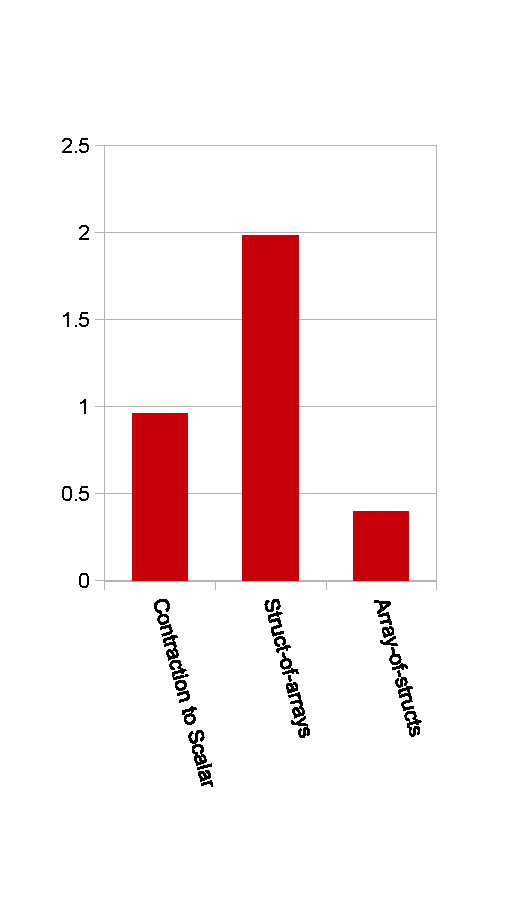
\includegraphics[scale=0.7]{./figures/perf2.pdf}
 \caption{Speedup of \framework over Halide for different data-layouts in an image processing pipeline}
 \label{fig:speedup2}
\end{figure}

Figure~\ref{fig:speedup2} shows the speedup of code generated from Halide-\framework over code generated from Halide-original for different data layouts.  We map the computations of an image processing pipeline to three different data-layouts: full contraction to scalars, struct-of-arrays and array-of-structs.  The goal of this experiment is not to evaluate the gains in performance but rather to show that \framework can actually perform data-layout transformations such as mapping to SOA, AOS and contraction.


%%%%%%%%%%%%%%%%%%%%

The \emph{Recursive Edge Detector} benchmark cannot be implemented in Halide given that it has a recursive definition (Halide does not allow recursive definitions).  Thus we implement the baseline for this benchmark in C rather than Halide.  That C code has two loop nests, the two loop nests can be parallelized but such a parallelism does not provide the best data locality.  In order to get both parallelism and data locality, we need to exploit wavefront parallelism by skewing the iteration space.  Expressing skewing in Halide is challenging since Halide uses an interval based representation in which expressing skewing is not trivial.  The \framework framework uses a polyhedral-based representation that is more expressive than the interval based representation used within Halide and thus \framework can easily express and apply skewing.
When we apply skewing in \framework, the code generated by Halide-\framework is $10.5\times$ faster than the sequential C code and is $2.7\times$ faster than the parallel C code (parallelization without skewing).  This benchmark shows that skewing in this case is good for performance since it enhances both data locality and
parallelism.
The benchmark also provides an example of a complex quasi-affine transformation of the iteration space that is not currently supported by Halide.  This shows the ability of \framework to express complex affine loop nest transformations.

%%%%%%%%%%%%%%%%%%%%


\begin{figure*}[t!]
    \centering
    \scriptsize
\begin{tabular}{cl|@{}l}
\multicolumn{3}{c}{\textbf{Constraints:} \boldsymbol{$\ \ \ C_n: 0\leq i < N, \ \ \ \ \ \ C_m: 0\leq j < M, \ \ \ \ C_{m'}: 1\leq j < M-1, \ \ \ \ C_{k}: 0\leq k < 3$}}
\\\hline
  &
    \ \ \ \ \ \ \ \ \ \ \ \ \ \ \ \ \ \ \ \ \ \ \ 
    \textbf{Different Code Optimizations}
  &
    \ \ \ \ \ \ \ \ \ \ \ \ \ \  
    \textbf{\framework representation (Layer I, Layer II and Layer III)}
\\\hline

{\textbf{\normalsize(a)}} &
\begin{lstlisting}[language=C,escapechar=@]
float b1[M][3], b2[M][3], img[N][M][3]
for (i in 0..N)
 for (j in 0..M)
  for (c in 0..2)
   b1[j][c] = 1.5*img[i][j][c]@\label{fig:motivating:code1:stmt1}@
 for (j in 0..M )
  for (c in 0..2)
   b2[j][c] = clamp(b1[j][c], 0, 255)@\label{fig:motivating:code1:stmt2}@
 for (j in 1..M-1)
  for (c in 0..2)
   out[i][j][c] = (b2[j-1][c] + b2[j][c] + 3@\label{fig:motivating:code1:stmt3}@
                 b2[j+1][c])/
\end{lstlisting}
    &  
\begin{tabular}{c|l}
\multirow{4}{*}{\textbf{Layer I}}
    & In the following, we use $C_n$, $C_m$ and $C_k$ which are defined above.\\
    & {\boldsymbol{$\{b_1\ (i, j, c): C_n \wedge C_m \wedge C_k\} $}}: $1.5*img(i, j, c)$\\
    & {\boldsymbol{$\{b_2\ (i, j, c): C_n \wedge C_m  \wedge C_k\}$}}: $\ clamp(b_1(i, j, c), 0, 255)$ \\
    & {\boldsymbol{$\{out(i, j, c): C_n \wedge C_m \wedge C_k\}$}}: $(b_2(i,j-1,c)+b_2(i,j,c)+b_2(i,j+1,c))/3$ \\\hline
\multirow{4}{*}{\textbf{Layer II}}
    & $\{\ b_1[0, i (cpu), j, c]: C_n \wedge C_m \wedge C_k\}: 1.5*img[i, j, c]$\\
    & $\{\ b_2[1, i (cpu), j, c]: C_n \wedge C_m \wedge C_k\}: clamp(b_1[0, i, j, c], 0, 255)$\\
    &$\{out[2, i (cpu), j, c]: C_n\wedge C_{m'} \wedge C_k \}:$\\
    &$(b_2[1,i,j-1,c]+b_2[1,i,j,c]+b_2[1,i,j+1,c])/3$\\\hline
\multirow{4}{*}{\textbf{Layer III}}
    & Layer II representation + the following data \ mapping\\
    & $\{\ b_1[1, i, 0, j, c] \rightarrow buf_{b1}[j,c]:  C_n \wedge C_m \wedge C_k\} $ \color{listinggreen}{ /* $C_n$, $C_m$ and $C_k$ are defined above. */} \\
    & $\{\ b_2[1, i, 1, j, c] \rightarrow buf_{b2}[j,c]:  C_n \wedge C_m \wedge C_k\}$\\
    & $\{out[1, i, 2, j, c] \rightarrow buf_{out}[i,j,c]:  C_n \wedge C_m \wedge C_k\}$\\
\end{tabular}
    \\\hline
{\textbf{\normalsize(b)}} &
\begin{lstlisting}[language=C,escapechar=@]
float b1[N][M][3], b2[N][M][3], img[N][M][3]
for (i in 0..N) // Parallel on CPU
 for (j in 0..M)
  for (c in 0..2)
   b1[i][j][c] = 1.5*img[i][j][c]@\label{fig:motivating:code2:stmt1}@
   b2[i][j][c] = clamp(b1[i][j][c], 0, 255)@\label{fig:motivating:code2:stmt2}@
 for (j in 1..M-1)
  for (c in 0..2)
   out[i][j][c] = (b2[i][j-1][c] + b2[i][j][c] +@\label{fig:motivating:code2:stmt3}@
                   b2[i][j+1][c])/3
\end{lstlisting}
    & 
\begin{tabular}{c|l}
 \multirow{2}{*}{\textbf{Layer I }}  & \\ & Same as Layer I in (a)\\ \\\hline
 \multirow{4}{*}{\textbf{Layer II}}
    & $\{\ b_1[0, i (cpu), j, c, 0]: C_n \wedge C_m \wedge C_k\}: 1.5*img[i, j, c]$\\
    & $\{\ b_2[0, i (cpu), j, c, 1]: C_n \wedge C_m \wedge C_k\}: clamp(b_1[0, i, j, c], 0, 255)$\\
    &$\{out[1, i (cpu), j, c, 0]: C_n\wedge C_{m'} \wedge C_k \}:$\\
    &$(b_2[0,i,j-1,c,0]+b_2[0,i,j,c,1]+b_2[1,i,j+1,c,0])/3$\\\hline
 \multirow{4}{*}{\textbf{Layer III}}
    & Layer II representation + the following data \ mapping\\
    & $\{b_1\ [0, i (cpu), j, c, 0] \rightarrow buf_{b1}[i,j,c]: C_n \wedge C_m \wedge C_k\}$\\
    & $\{b_2\ [0, i (cpu), j, c, 1] \rightarrow buf_{b2}[i,j,c]: C_n \wedge C_m \wedge C_k\}$\\
    & $\{out[1, i (cpu), j, c, 0] \rightarrow buf_{out}[i,j,c]: C_n \wedge C_{m'} \wedge C_k\}$\\\hline
\end{tabular}  
    \\\hline
    {\textbf{\normalsize(c)}} &
\begin{lstlisting}[language=C,escapechar=@]
float b1[N][M][3], b2[N][M][3], img[N][M][3]
for (i in 0..N) // Parallel on GPU
 for (j in 0..M)
  for (c in 0..2)
   float t = 1.5*img[i][j][c]@\label{fig:motivating:code2:stmt1}@
   b2[i][j][c] = clamp(t, 0, 255)@\label{fig:motivating:code2:stmt2}@
 for (j in 1..M-1)
  for (c in 0..2)
   out[i][j][c] = (b2[i][j-1][c] + b2[i][j][c] +@\label{fig:motivating:code2:stmt3}@
                   b2[i][j+1][c])/3
\end{lstlisting}
    & 
\begin{tabular}{c|l}
 \multirow{4}{*}{\textbf{Layer I }}  & \\ & Same as Layer I in (a)\\ \\\hline
 \multirow{2}{*}{\textbf{Layer II}}
    & \\ & Same as Layer II in (b)\\\hline
 \multirow{4}{*}{\textbf{Layer III}}
    & \\ & Same as Layer III in (b) except the mapping of $b_1$ and $b_2$ which should be replaced with \\ \\
    & $\{b_1\ [0, i (cpu), j, c, 0] \rightarrow t: C_n \wedge C_m \wedge C_k\}$\\
    & $\{\ \ b_2[0, i (gpu), j, c, 1] \rightarrow buf_{b2}[c,i,j]:  C_n \wedge C_m \wedge C_k\}$\\
\end{tabular}
    \\\hline
{\textbf{\normalsize(d)}} &
\begin{lstlisting}[language=C,escapechar=@]
float b2[3][3], img[N][M][3]
for (i in 0..N) // Parallel on CPU
 for (j in 0..M)
  for (c in 0..2)
   b2[j%3][0] = clamp(1.5*img[i][j-1][c], 0, 255)
   b2[j%3][1] = clamp(1.5*img[i][j][c], 0, 255)
   b2[j%3][2] = clamp(1.5*img[i][j+1][c], 0, 255)
   if (j>=3)
     img[i][j-2][c] = (b2[(j-2)%3][0] + 
                       b2[(j-2)%3][1] +
                       b2[(j-2)%3][2])/3
 img[i][M-2][c] = (b2[(M-2)%3][0]+b2[(M-2)%3][1]+
                   b2[(M-2)%3][2])/3
 img[i][M-1][c] = (b2[(M-1)%3][0]+b2[(M-1)%3][1]+
                   b2[(M-1)%3][2])/3
\end{lstlisting}
    & 
\begin{tabular}{c|l}
 \multirow{4}{*}{\textbf{Layer I }}  & \\ & Same as Layer I in (a)\\ \\\hline
 \multirow{8}{*}{\textbf{Layer II}}
                & $\{\ b_2[0, i (cpu), j, c]: C_n \wedge C_m \wedge C_k\}:clamp(1.5*img[i, j-1, c], 0, 255)$\\
                & $\{\ b_2[1, i (cpu), j, c]: C_n \wedge C_m \wedge C_k\}:clamp(1.5*img[i, j, c], 0, 255)$\\
                & $\{\ b_2[2, i (cpu), j, c]: C_n \wedge
                C_m \wedge C_k\}:clamp(1.5*img[i, j+1, c], 0, 255)$\\
                &$\{img[3, i (cpu), j+2, c]:C_n\wedge C_{m'} \wedge C_k\}:$\\
                & $(b_2[0,i,j+1,c]+
                b_2[1,i,j+2,c]+b_2[2,i,j+3,c])/3$\\\hline
 \multirow{8}{*}{\textbf{Layer III}}
    & Layer II representation + the following data mapping\\
    & We assume that $buf_{b2}$ is allocated locally in each processor\\
    &  $\{b_2\ [k, i (cpu), j, c] \rightarrow buf_{b2}[j\%3,c]: C_n \wedge C_m \wedge C_k\}$\\
    &  $\{img\ [3, i (cpu), j, c] \rightarrow buf_{img}[i, j, c]: C_n \wedge C_m \wedge C_k\}$\\
    \\\hline
 \end{tabular} 
    \\
    \end{tabular}
    \caption{Resulting code and the three layers of representation for 
    (a) Unoptimized code implementing the motivating example,
    (b) Full expansion of b1 and b2 to allow parallelism and loop fusion,
    (c) Contraction of b1 to a scalar,
    (d) Storage of b2 in a struct-of-arrays (SOA), and 
    (e) Fusion with redundant computation and shifting. }
    \label{fig:example-ir}
\end{figure*}

%%%%%%%%%%%%%%%%%%%

\HIDE{
\vspace{-0.25cm}
\subsection{The Necessity of a Multi-layer IR}

Compiler middle-ends need to schedule the iteration domain onto a modern architecture to take advantage of available parallelism and manage the complex memory hierarchy.
In many cases, it is difficult to know the best data-mapping before deciding how to schedule a program.  Consider the simple image processing pipeline in Figure~\ref{fig:example-ir}-\codeone{} (left).
%It takes as input a three-channel (RGB) image produced by an earlier image processing stage, brightens it, ensuring that the value remains representable by an 8-bit value, and then blurs the brightened image using a horizontal average blur filter.
We use this example to demonstrate that the optimal data layout for intermediates depends on the schedule and target architecture. Expressing these different data layouts and schedules for the same algorithm in order to target different architectures is made easy thanks to the three-layer design of \framework{} which separates the algorithm from the schedule and data layout specifications.

%**********************************************************************************

% \codeone{} Full expansion of b1 and b2 to allow parallelism;
% \codetwo{} Loop fusion + contraction of b1 to a scalar;
% \codethree{} Loop fusion + Transformation to AOS (Array Of Structures) for GPU execution;
% \codefour{} Loop fusion + redundant computation; and
% \codefive{} Loop fusion + redundant computation + shifting + inplace computation}



Code in Figure~\ref{fig:example-ir}-\codeone{} is not optimized.  In order to optimize it for a multicore machine, we can parallelize of the outermost loop (over the \lstinline{i} iterator).  To do so, we must first expand the two-dimensional arrays \lstinline{b1} and~\lstinline{b2} into three-dimensional arrays.  In addition to the parallelization, data locality can be improved by fusing the brightening and clamp stages.  After applying these optimizations, we get the code shown in Figure~\ref{fig:example-ir}-\codetwo{} (left).  
Assuming now that the target architecture is a GPU instead of a CPU, changing from a Structure-of-Arrays (SoA) memory layout to an Array-of-Structures (AoS) layout may lead to better performance.
Another optimization would be to replace the \lstinline{b1} array accesses with accesses to a scalar.
In order to parallelize the two outermost loops, the loop over \lstinline{b2} and the loop over \lstinline{out} can be distributed.  The result of applying these optimizations is shown in Figure~\ref{fig:example-ir}-\codethree{} (left).

%To maximize parallelism and data locality, we should fuse all loops of the pipeline.  This fusion is possible, but requires introducing redundant computation.  Since only 3 elements of \lstinline{b2} are computed and then immediately consumed in each iteration of the \lstinline{c} loop, we contract the array \lstinline{b2} into just an array of three elements.  In order to further reduce the memory footprint, we use in-place computations: we write the output of the pipeline directly in the input \lstinline{img[]} buffer.  In order for the fusion to be valid in this case, we must shift the computation of the output by 2 iterations so that all of the input \lstinline{img[]} pixels are consumed before being overwritten by the output of the pipeline. Figure~\ref{fig:example-ir}-\codefour{} shows the resulting code.

These examples show that there is a need for an intermediate representation that avoids committing to a specific data layout at an early stage, since sometimes it is advantageous and easier to perform data layout mapping only after deciding on the computation schedule, target architecture and composition with other computations (producer-consumer relationship).  It also shows that different hardware architecture require different schedules. Thus, a middle-end compiler that targets multiple hardware architectures should allow the user to easily try different schedules and data mappings.  Such exploration becomes easy with the separation of the three layers (algorithm, schedule and data-layout layers).

%This example also shows that a middle-end compiler needs a flexible and powerful framework for code transformation since it is challenging to correctly perform advanced loop nest transformations such as loop fusion, loop shifting, the introduction of redundant computations.
}

%%%%%%%%%%%%%%%%%%%%%%%%%